\documentclass[fonts]{icst}

\usepackage[breaklinks,colorlinks,bookmarksopen,bookmarksnumbered,linkcolor=ICSTblue,citecolor=blue,urlcolor=ICSTblue]{hyperref}
\usepackage{breakurl}
\usepackage{doi}
\usepackage{graphicx,color,flushend}
\usepackage{amsmath,amssymb}
\usepackage{booktabs}
\usepackage{tikz}
\usetikzlibrary{arrows.meta,positioning}

\def\volumeyear{2026}
\journalname{EAI Endorsed Transactions on Scalable Information Systems}
\articletype{Research Article}
\setcounter{page}{01}
\def\volumenumber{XX}
\def\issuemonth{XX-XX}
\def\issuenumber{X}
\def\articleid{XX}
\def\copyrightholder{Joseph Raj \textit{et al.}, licensed to EAI}
\copyrightnote{This is an open access article distributed under the terms of the Creative Commons Attribution license (\url{http://creativecommons.org/licenses/by/3.0/}), which permits unlimited use, distribution and reproduction in any medium so long as the original work is properly cited.}
\def\articledoi{10.4108/XX.X.X.XX}
\received{XXXX}
\accepted{XXXX}
\published{XXXX}

\begin{document}

\runningheads{J. Raj et al.}{Stock Market Index Direction Prediction Using Limit Order Book Data}

\title{Stock Market Index Direction Prediction Using Limit Order Book Data}

\author{Joseph Raj\affil{1}\fnoteref{1}, Sumanth G.~M\affil{1}, Abhishek Kumar\affil{1}, Kumara Swamy\affil{1}, Raghav\affil{1}, Saagar\affil{1}}

\address{\affilnum{1} Department of Data Science, Machine Learning \& Artificial Intelligence, PES University, Bengaluru, Karnataka -- 560100, India}

\abstract{
Short-horizon prediction of mid-price direction from Limit Order Book (LOB) data is a central problem in
market microstructure, but research is concentrated on developed markets and the public FI-2010 benchmark.
We address two gaps. First, a \emph{data-engineering} gap: because no clean Indian index-futures LOB dataset
existed, we reverse-engineered the undocumented Dhan twenty-level binary depth feed, built a cloud collection
pipeline (an EC2 WebSocket collector writing daily Parquet to Amazon S3) with automated token refresh and
contract-expiry handling, and produced a continuous front-month series for NIFTY and BANKNIFTY index futures
($\approx$1.1\,million events per instrument) aligned to the FI-2010 contract. Second, a \emph{modelling}
gap: we introduce \textbf{MambaLOB}, a selective state-space (SSM) architecture with linear-time $O(L)$
scaling, and a convolutional hybrid \textbf{ConvMambaLOB}, and compare them against reproduced DeepLOB,
MLPLOB and TLOB baselines under one protocol. We further engineer microstructure features (order-flow
imbalance, micro-price, depth imbalance, and a broker-unique order-count channel) and validate every claim
with multi-seed confidence intervals, paired significance tests, calibration, and hyperparameter
optimisation. The headline result is reported honestly: the SSM models recover roughly 90\% of the
transformer's accuracy at $12$--$25\times$ fewer parameters --- an efficiency result rather than an accuracy
win --- while microstructure feature engineering, not architecture, drives the only statistically significant
improvement on the Indian market.
}

\keywords{Limit Order Book, Mid-price Prediction, State-Space Models, Mamba, Market Microstructure, NSE Index Futures, Deep Learning, Data Engineering}

\fnotetext[1]{Corresponding author. Email: \email{rajjoseph48@gmail.com}}

\maketitle

% =====================================================================
\section{Introduction}
Electronic exchanges operate as continuous double auctions whose state is recorded in a Limit Order Book
(LOB): the set of outstanding bid and ask orders at each price level. The LOB carries a rich microstructural
signal for short-horizon price prediction, and deep learning models have shown small but real predictive
power on it. However, this research is concentrated on developed markets (NASDAQ, Nordic exchanges) and on
the single public benchmark, FI-2010~\cite{fi2010}. Indian index futures are highly liquid yet structurally
distinct (tick discreteness, regime shifts, distinct liquidity profiles) and remain almost entirely unstudied
with modern LOB architectures.

Index direction is hard to predict because the series is non-stationary and governed by rapidly evolving
supply--demand dynamics. The order book updates irregularly and at high frequency, yet most prior deep LOB
models train on coarse fixed-grid snapshots (e.g.\ one-second sampling) that lose intra-interval dynamics. We
capture NSE depth at the broker's native push cadence ($\approx$2.5\,Hz), finer-grained than typical
one-second snapshots, while noting transparently that this remains a near-regular snapshot feed rather than
tick-by-tick data.

This paper makes the following contributions:
\begin{itemize}
\item \textbf{An engineered NSE index-futures LOB dataset.} To our knowledge the first ML-ready Indian
index-futures LOB dataset, built end-to-end from the reverse-engineered Dhan binary feed through a documented
cloud pipeline and a front-month stitching/preprocessing pipeline aligned to FI-2010.
\item \textbf{MambaLOB and ConvMambaLOB.} A selective state-space architecture for LOB direction
classification and a convolutional hybrid, with a rigorous efficiency comparison ($O(L)$ vs.\ $O(L^2)$).
\item \textbf{Microstructure feature engineering.} Engineered order-flow imbalance, micro-price, depth
imbalance, and a broker-unique order-count channel, shown to give a statistically significant gain.
\item \textbf{An honest transfer and rigour study.} A standardized comparison of four architectures on the
NSE benchmark with multi-seed significance, calibration, and hyperparameter optimisation, and transparent
reporting of what does and does not transfer from FI-2010.
\end{itemize}

% =====================================================================
\section{Related Works}
\subsection{Classical techniques}
Parametric time-series models (AR, ARMA, ARIMA) and Hidden Markov Models were first applied to price
forecasting. They model only the derived price/return series, ignore book depth, and fail under the
non-linear, non-stationary behaviour of high-frequency LOB data; they serve only as conceptual baselines.

\subsection{The FI-2010 benchmark and CNN--LSTM models}
FI-2010~\cite{fi2010} is the first public LOB benchmark --- ten levels of depth for five Nasdaq Nordic stocks
over ten days --- providing normalised feature variants, a smoothed mid-price labelling rule at horizons
$k\in\{10,20,50,100\}$, and standard cross-folds. DeepLOB~\cite{deeplob} is the seminal deep model: a
convolutional stack that fuses price/volume then book sides, an Inception module for multi-scale temporal
patterns, and an LSTM. It established the interleaved 40-feature $\times$ window representation that all
subsequent work (including ours) adopts, but is limited by its sequential LSTM and lack of attention.

\subsection{Transformer and state-space models}
MLPLOB and TLOB~\cite{tlob} reframe LOB models as stacks of normalization-plus-mixing blocks; TLOB uses
\emph{dual} (temporal and feature) self-attention and is the current state of the art on FI-2010. Structured
state-space models --- S4~\cite{s4} and the selective-scan Mamba~\cite{mamba} --- offer sub-quadratic and
linear-time sequence modelling competitive with transformers. Their use as a discriminative classification
backbone for LOB direction is the gap this work targets.

\subsection{Benchmark studies and microstructure priors}
The LOBCAST benchmark study~\cite{lobcast} re-implemented fifteen deep LOB models and found they overfit
FI-2010 and degrade sharply on unseen data --- motivating our honest transfer framing and dual-metric
reporting. Independently, the microstructure literature supplies strong priors: order-flow imbalance is a
robust predictor of short-horizon moves~\cite{ofi}, and the micro-price~\cite{microprice} is a volume-weighted
fair-value estimator superior to the mid. These underpin our engineered features.

% =====================================================================
\section{Methodology}
\subsection{Engineered NSE dataset and data pipeline}
Because no clean Indian index-futures LOB dataset existed, the dataset was engineered end to end. The Dhan
twenty-level depth WebSocket delivers an \emph{undocumented binary frame}, which we decoded offline: a
1992-byte full format (a 40-byte header followed by twenty 16-byte bid and twenty 16-byte ask records of
order-count, price, and quantity) and a 664-byte compact format. Decoding required fixing non-obvious issues
--- the bid price sits at byte offset $+4$, empty levels emit denormalised near-zero floats that must be
rejected, and quantity/order-count fields overflow 32-bit integers (we store \texttt{int64}). A lightweight
EC2 collector subscribes to the NIFTY and BANKNIFTY near-month futures on the \texttt{NSE\_FNO} segment,
writes one row per server push to daily \texttt{zstd} Parquet, and a cron job syncs to S3 after the close. The
May contract expired during collection; the loader stitches the May and June contracts into one continuous
front-month series by root symbol, treating the roll (and every overnight gap) as a segment boundary. The
result is 21 valid trading days (12 May -- 12 June 2026), $\approx$57{,}000 events/instrument/day
($\approx$1.1\,M per instrument, exceeding FI-2010's $\approx$400\,k scale). Figure~\ref{fig:pipeline}
summarises the end-to-end data-engineering flow.

\begin{figure*}[t]
\centering
\resizebox{0.92\textwidth}{!}{%
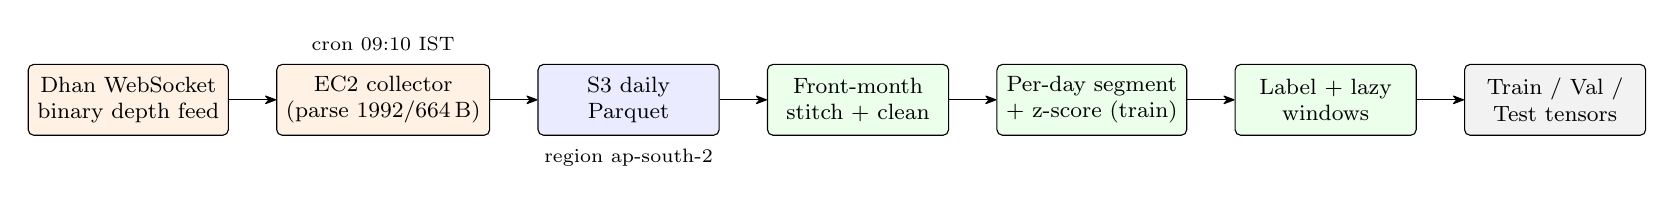
\begin{tikzpicture}[
  font=\footnotesize, >={Stealth[round]}, node distance=6mm,
  stage/.style={draw, rounded corners=2pt, align=center, minimum height=9mm, minimum width=23mm},
  acq/.style={stage, fill=orange!10}, store/.style={stage, fill=blue!8},
  prep/.style={stage, fill=green!8}, result/.style={stage, fill=gray!10}]
\node[acq] (dhan) {Dhan WebSocket\\binary depth feed};
\node[acq, right=of dhan] (ec2) {EC2 collector\\(parse 1992/664\,B)};
\node[store, right=of ec2] (s3) {S3 daily\\Parquet};
\node[prep, right=of s3] (stitch) {Front-month\\stitch + clean};
\node[prep, right=of stitch] (seg) {Per-day segment\\+ z-score (train)};
\node[prep, right=of seg] (lab) {Label + lazy\\windows};
\node[result, right=of lab] (ds) {Train / Val /\\Test tensors};
\draw[->] (dhan)--(ec2); \draw[->] (ec2)--(s3); \draw[->] (s3)--(stitch);
\draw[->] (stitch)--(seg); \draw[->] (seg)--(lab); \draw[->] (lab)--(ds);
\node[font=\scriptsize, above=0.5mm of ec2] {cron 09:10 IST};
\node[font=\scriptsize, below=0.5mm of s3] {region ap-south-2};
\end{tikzpicture}}
\caption{Engineered NSE data pipeline. The reverse-engineered Dhan binary feed (1992\,B full / 664\,B compact
frames) is parsed on an EC2 collector and written as daily Parquet to S3; the modelling layer then stitches
the front-month series across the expiry roll, cleans, segments per trading day, z-scores on training
statistics, labels, and emits lazily-windowed tensors aligned to FI-2010.}
\label{fig:pipeline}
\end{figure*}

\subsection{Preprocessing and labelling}
The pipeline (i) stitches the front-month series, (ii) reorders Dhan's columns to the interleaved FI-2010
layout $[P^a_i,V^a_i,P^b_i,V^b_i]\times 10$, (iii) cleans crossed quotes and tick spikes, (iv) segments per
trading day so labels and windows never cross a day/contract boundary, (v) z-scores using \emph{training}
statistics only, and (vi) forms lazy sliding windows of length $L=100$. Labels follow the FI-2010 smoothed-mid
convention: with $m^-,m^+$ the mean mid over the $k$ events behind/ahead and $r=(m^+-m^-)/m^-$, the label is
Up if $r>\alpha$, Down if $r<-\alpha$, else Stationary, with a fixed $\alpha=10^{-5}$ calibrated for the
index-futures price scale.

\subsection{Microstructure feature engineering}
On top of the raw 40-feature vector we engineer microstructure channels: order-flow imbalance (OFI) at
level~1 and summed over levels 1--5 (segment-aware), the micro-price
$p_{\mathrm{micro}}=\tfrac{V_1^b P_1^a + V_1^a P_1^b}{V_1^a+V_1^b}$, relative spread, depth imbalance, and the
\emph{Dhan-unique per-level order count}. These define feature sets used for ablation: \texttt{base40} (raw),
\texttt{micro} (+6 scalars), \texttt{orders60}, \texttt{depth80} (20 levels), and \texttt{all} (66 features).

\subsection{Models}
All models share a $(B,100,40)\!\rightarrow\!\mathbb{R}^3$ contract and are compared under one protocol. We
reproduce three baselines (Figure~\ref{fig:baselines}): \textbf{DeepLOB} (CNN+Inception+LSTM)~\cite{deeplob},
\textbf{MLPLOB} (MLP + Bilinear Normalization, the ablation floor), and \textbf{TLOB} (dual-attention
transformer, the SOTA reference, vendored faithfully)~\cite{tlob}.

\begin{figure*}[t]
\centering
\resizebox{0.95\textwidth}{!}{%
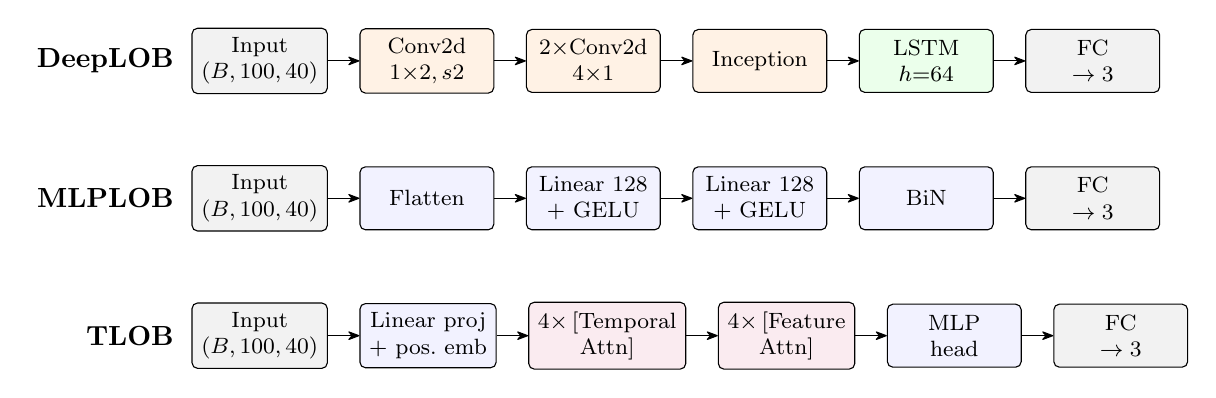
\begin{tikzpicture}[
  font=\footnotesize, >={Stealth[round]}, node distance=4mm,
  b/.style={draw, rounded corners=2pt, align=center, minimum height=8mm, minimum width=17mm, fill=blue!5},
  io/.style={b, fill=gray!10}, conv/.style={b, fill=orange!10}, attn/.style={b, fill=purple!8},
  rec/.style={b, fill=green!8}]
\node[io] (d0) {Input\\$(B,100,40)$};
\node[conv, right=of d0] (d1) {Conv2d\\$1{\times}2,s2$};
\node[conv, right=of d1] (d2) {$2{\times}$Conv2d\\$4{\times}1$};
\node[conv, right=of d2] (d3) {Inception};
\node[rec, right=of d3] (d4) {LSTM\\$h{=}64$};
\node[io, right=of d4] (d5) {FC\\$\to 3$};
\foreach \a/\b in {d0/d1,d1/d2,d2/d3,d3/d4,d4/d5} \draw[->] (\a)--(\b);
\node[left=1mm of d0, font=\bfseries] {DeepLOB};
\node[io, below=9mm of d0] (m0) {Input\\$(B,100,40)$};
\node[b, right=of m0] (m1) {Flatten};
\node[b, right=of m1] (m2) {Linear 128\\+ GELU};
\node[b, right=of m2] (m3) {Linear 128\\+ GELU};
\node[b, right=of m3] (m4) {BiN};
\node[io, right=of m4] (m5) {FC\\$\to 3$};
\foreach \a/\b in {m0/m1,m1/m2,m2/m3,m3/m4,m4/m5} \draw[->] (\a)--(\b);
\node[left=1mm of m0, font=\bfseries] {MLPLOB};
\node[io, below=9mm of m0] (t0) {Input\\$(B,100,40)$};
\node[b, right=of t0] (t1) {Linear proj\\+ pos.\ emb};
\node[attn, right=of t1] (t2) {$4{\times}$\,[Temporal\\Attn]};
\node[attn, right=of t2] (t3) {$4{\times}$\,[Feature\\Attn]};
\node[b, right=of t3] (t4) {MLP\\head};
\node[io, right=of t4] (t5) {FC\\$\to 3$};
\foreach \a/\b in {t0/t1,t1/t2,t2/t3,t3/t4,t4/t5} \draw[->] (\a)--(\b);
\node[left=1mm of t0, font=\bfseries] {TLOB};
\end{tikzpicture}}
\caption{Reproduced baseline architectures, all sharing the $(B,100,40)\!\to\!3$ contract: DeepLOB
(CNN+Inception+LSTM), MLPLOB (flatten+MLP with Bilinear Normalization, the ablation floor), and TLOB
(alternating temporal and feature self-attention, the transformer SOTA).}
\label{fig:baselines}
\end{figure*}

The proposed \textbf{MambaLOB} (Figure~\ref{fig:arch}) projects the LOB window to $d_{\mathrm{model}}$ and
applies $n$ selective state-space blocks (Figure~\ref{fig:mambablock}) realising an input-dependent linear
recurrence
\begin{equation}
h_t = \bar{A}_t\,h_{t-1} + \bar{B}_t\,x_t, \qquad y_t = C_t\,h_t,
\end{equation}
where $\bar A,\bar B,C$ depend on the input (the selection mechanism), giving $O(L)$ time and memory and a
parameter count independent of $L$. \textbf{ConvMambaLOB} prepends DeepLOB's convolutional spatial front-end
to the Mamba core, replacing the sequential LSTM with the selective SSM.

\begin{figure}[t]
\centering
\resizebox{\linewidth}{!}{%
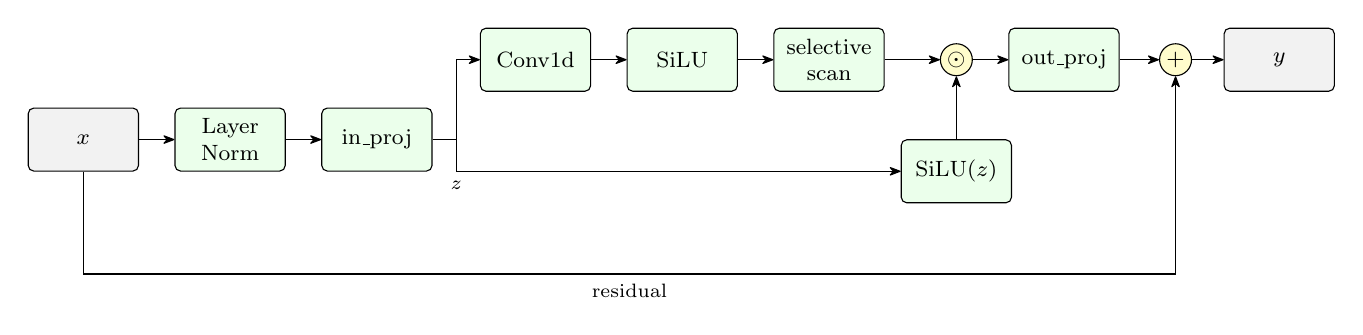
\begin{tikzpicture}[
  font=\footnotesize, >={Stealth[round]}, node distance=4.5mm,
  b/.style={draw, rounded corners=2pt, align=center, minimum height=8mm, minimum width=14mm, fill=green!8},
  op/.style={draw, circle, inner sep=1pt, fill=yellow!20}, io/.style={b, fill=gray!10}]
\node[io] (x) {$x$};
\node[b, right=of x] (norm) {Layer\\Norm};
\node[b, right=of norm] (inproj) {in\_proj};
\node[b, above right=2mm and 6mm of inproj] (conv) {Conv1d};
\node[b, right=of conv] (silu) {SiLU};
\node[b, right=of silu] (scan) {selective\\scan};
\node[op, right=7mm of scan] (gate) {$\odot$};
\node[b, below=8mm of gate] (z) {SiLU$(z)$};
\node[b, right=of gate] (outproj) {out\_proj};
\node[op, right=5mm of outproj] (add) {$+$};
\node[io, right=4mm of add] (y) {$y$};
\draw[->] (x)--(norm); \draw[->] (norm)--(inproj);
\draw[->] (inproj.east) -- ++(3mm,0) |- (conv.west);
\draw[->] (inproj.east) -- ++(3mm,0) |- (z.west) node[midway,below,font=\scriptsize]{$z$};
\draw[->] (conv)--(silu); \draw[->] (silu)--(scan); \draw[->] (scan)--(gate);
\draw[->] (z)--(gate); \draw[->] (gate)--(outproj); \draw[->] (outproj)--(add); \draw[->] (add)--(y);
\draw[->] (x.south) |- ++(0,-13mm) -| (add.south) node[near start,below,font=\scriptsize]{residual};
\end{tikzpicture}}
\caption{The selective state-space (Mamba) block: the input is normalised and split into two streams; one
passes a depthwise causal convolution and SiLU into the selective scan (input-dependent $\bar A,\bar B,C$),
the other forms the SiLU gate. The gated output is projected back and added to the residual; the scan is the
only sequential step and runs in $O(L)$.}
\label{fig:mambablock}
\end{figure}

\begin{figure}[t]
\centering
\resizebox{\linewidth}{!}{%
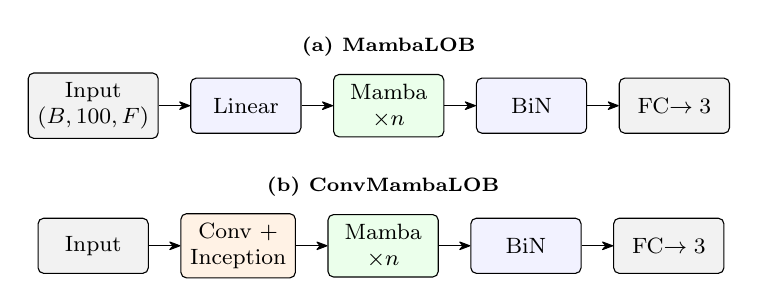
\begin{tikzpicture}[font=\footnotesize,>={Stealth[round]},node distance=4mm,
  b/.style={draw,rounded corners=2pt,align=center,minimum height=7mm,minimum width=14mm,fill=blue!5},
  m/.style={b,fill=green!8},c/.style={b,fill=orange!10},io/.style={b,fill=gray!10}]
\node[io](a0){Input\\$(B,100,F)$};
\node[b,right=of a0](a1){Linear};
\node[m,right=of a1](a2){Mamba\\$\times n$};
\node[b,right=of a2](a3){BiN};
\node[io,right=of a3](a4){FC$\to3$};
\foreach \x/\y in {a0/a1,a1/a2,a2/a3,a3/a4} \draw[->](\x)--(\y);
\node[above=1mm of a2,font=\scriptsize\bfseries]{(a) MambaLOB};
\node[io,below=10mm of a0](e0){Input};
\node[c,right=of e0](e1){Conv +\\Inception};
\node[m,right=of e1](e2){Mamba\\$\times n$};
\node[b,right=of e2](e3){BiN};
\node[io,right=of e3](e4){FC$\to3$};
\foreach \x/\y in {e0/e1,e1/e2,e2/e3,e3/e4} \draw[->](\x)--(\y);
\node[above=1mm of e2,font=\scriptsize\bfseries]{(b) ConvMambaLOB};
\end{tikzpicture}}
\caption{Proposed architectures. MambaLOB applies $n$ selective state-space blocks for $O(L)$ temporal mixing;
ConvMambaLOB prepends a convolutional spatial front-end before the Mamba core.}
\label{fig:arch}
\end{figure}

\subsection{Training and evaluation}
Training uses class-weighted cross-entropy, AdamW with cosine decay, and early stopping on validation
$F_1$. We report weighted and macro $F_1$ side by side (the FI-2010 headline is a \emph{weighted} $F_1$,
whereas independent reproductions report \emph{macro}), plus accuracy and Matthews correlation (MCC), against
naive majority/stationary/random baselines. The NSE split is chronological (train 12 May--4 June; test
5--12 June).

% =====================================================================
\section{Experiments and Results}
\subsection{FI-2010 reproduction}
Table~\ref{tab:fi2010} validates the pipeline: DeepLOB's weighted $F_1$ matches the paper's headline
($\approx$83\%) and TLOB reaches the SOTA range, confirming faithful reproductions before transfer.

\begin{table}[t]
\centering\footnotesize
\caption{FI-2010 (CF\_7, $L{=}100$): weighted / macro $F_1$ (\%).}
\label{tab:fi2010}
\begin{tabular}{@{}lcc@{}}
\toprule
Model & $k{=}10$ & $k{=}100$ \\
\midrule
DeepLOB       & 82.5 / 71.9 & --- \\
TLOB          & 88.0 / 81.1 & 92.5 / 92.5 \\
MambaLOB      & 79.2 / 67.4 & 69.3 / 68.7 \\
\bottomrule
\end{tabular}
\end{table}

\subsection{NSE transfer}
On the engineered NSE benchmark (Table~\ref{tab:nse}, Figure~\ref{fig:nse}) all models beat the naive
baselines, so learnable signal exists, but absolute scores fall well below FI-2010 --- the expected
degradation on new data, consistent with LOBCAST~\cite{lobcast}. TLOB leads throughout. The key transfer
finding for the proposed model: on NIFTY, MambaLOB (68k parameters) outperforms DeepLOB (191k) and matches
MLPLOB, second only to TLOB --- whereas on FI-2010 it trailed DeepLOB. The selective SSM thus transfers
\emph{better} to the Indian market, at $\approx$1/27 of TLOB's parameters.

\begin{table}[t]
\centering\footnotesize
\caption{NSE Scheme-A test weighted $F_1$ (range over $k\in\{10,20,50,100\}$). Lift = $F_1$ minus best naive baseline.}
\label{tab:nse}
\begin{tabular}{@{}lccc@{}}
\toprule
Model & NIFTY & BANKNIFTY & Lift \\
\midrule
DeepLOB         & 0.44--0.52 & 0.46--0.50 & 0.03--0.12 \\
MLPLOB          & 0.46--0.64 & 0.35--0.47 & 0.01--0.19 \\
MambaLOB        & 0.52--0.59 & 0.45--0.48 & 0.02--0.17 \\
\textbf{TLOB}   & \textbf{0.60--0.71} & \textbf{0.64--0.72} & \textbf{0.25--0.30} \\
\bottomrule
\end{tabular}
\end{table}

\begin{figure}[t]
\centering
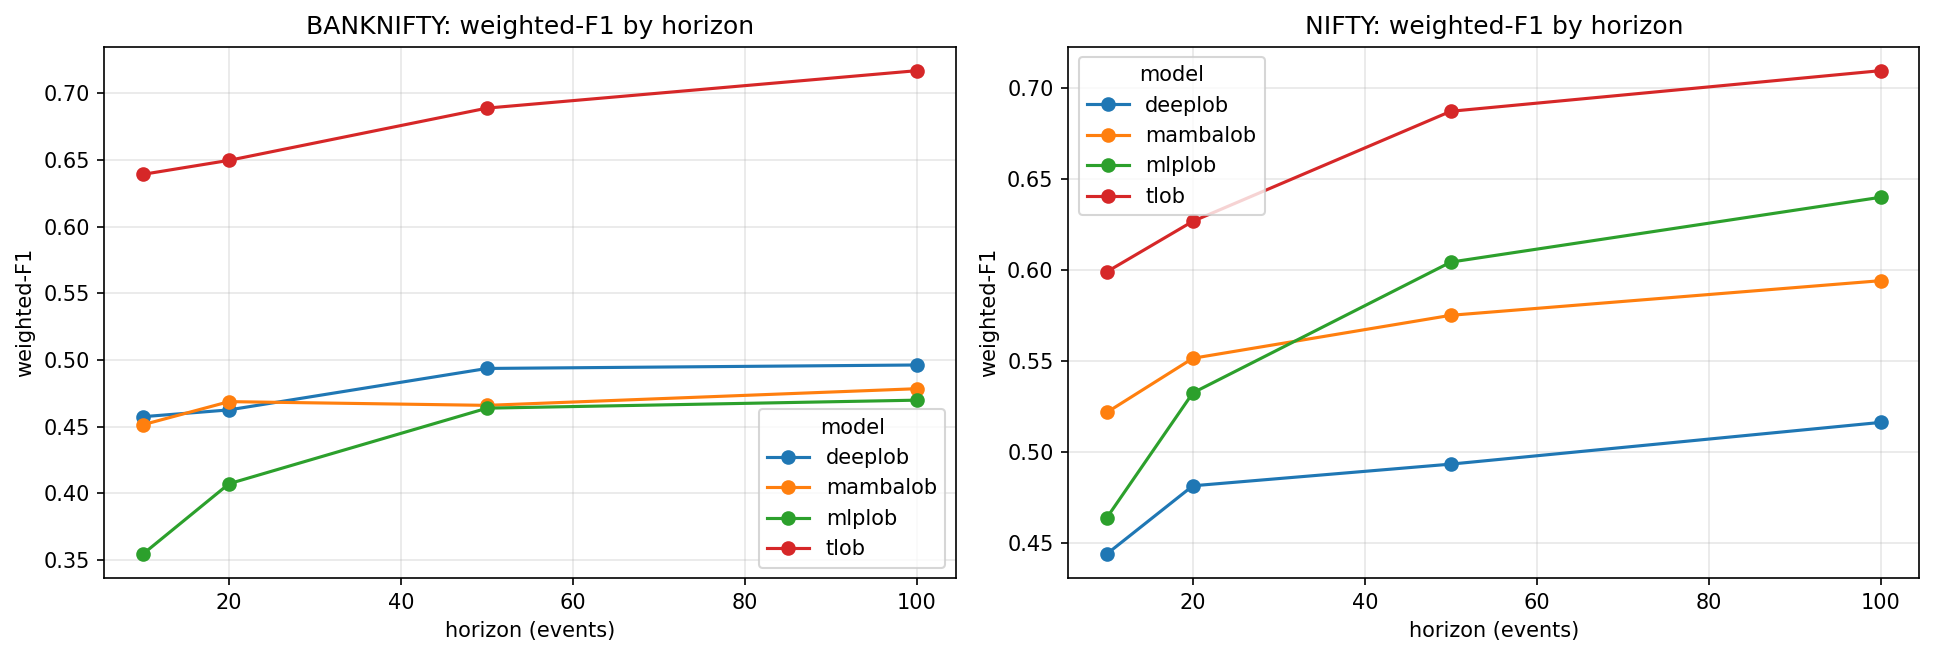
\includegraphics[width=\linewidth]{img/figures/nse_fig_nse_wf1_by_horizon.png}
\caption{NSE transfer (Scheme~A): test weighted-$F_1$ by horizon. TLOB leads; MambaLOB transfers competitively
on NIFTY at a fraction of the parameters.}
\label{fig:nse}
\end{figure}

\subsection{Feature engineering and improved architectures}
Microstructure feature engineering helps (Figure~\ref{fig:featabl}): the \texttt{all} set lifts MambaLOB's
weighted $F_1$ by up to $+0.068$ at $k{=}100$, with the gain growing with horizon, while deep levels and order
counts \emph{alone} do not help in isolation. For architecture (Table~\ref{tab:arch}, Figure~\ref{fig:scatter}),
ConvMambaLOB is the best of the proposed variants, but no Mamba variant beats TLOB on accuracy. The
contribution is the trade-off: \textbf{ConvMambaLOB recovers $\sim$90\% of TLOB's quality with $12.5\times$
fewer parameters}.

\begin{figure}[t]
\centering
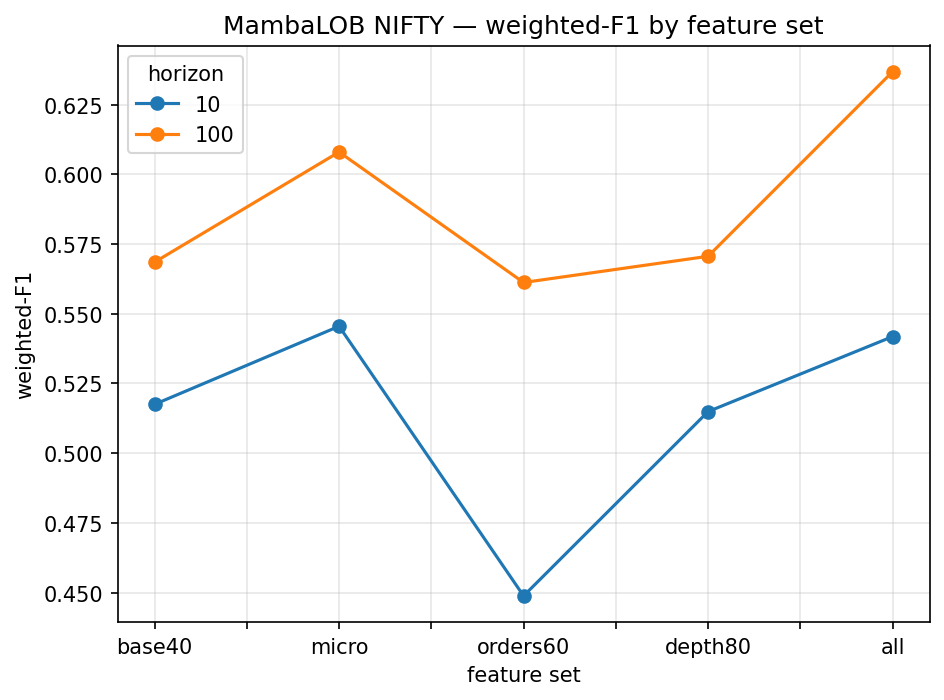
\includegraphics[width=\linewidth]{img/figures/feature_ablation_fig_feature_ablation.png}
\caption{Feature ablation (MambaLOB, NIFTY): weighted $F_1$ by feature set and horizon. The engineered
\texttt{micro} and \texttt{all} sets sit above the raw \texttt{base40}, with the gain widening at the longer
horizon; deep levels and order counts in isolation do not help.}
\label{fig:featabl}
\end{figure}

\begin{table}[t]
\centering\footnotesize
\caption{Architecture comparison (NIFTY+BANKNIFTY, mean over $k\in\{10,100\}$, \texttt{all} features).}
\label{tab:arch}
\begin{tabular}{@{}lcccc@{}}
\toprule
Model & Params & wF1 & mF1 & \% TLOB \\
\midrule
MambaLOB (base)        & \textbf{70k} & 0.595 & 0.508 & 89\% \\
\;+ bidirectional      & 135k & 0.597 & 0.509 & 90\% \\
\;+ Conv (ConvMambaLOB)& 144k & \textbf{0.602} & \textbf{0.518} & \textbf{90\%} \\
\;+ both               & 209k & 0.587 & 0.508 & 88\% \\
TLOB                   & 1.80M & \textbf{0.666} & \textbf{0.570} & 100\% \\
\bottomrule
\end{tabular}
\end{table}

\begin{figure}[t]
\centering
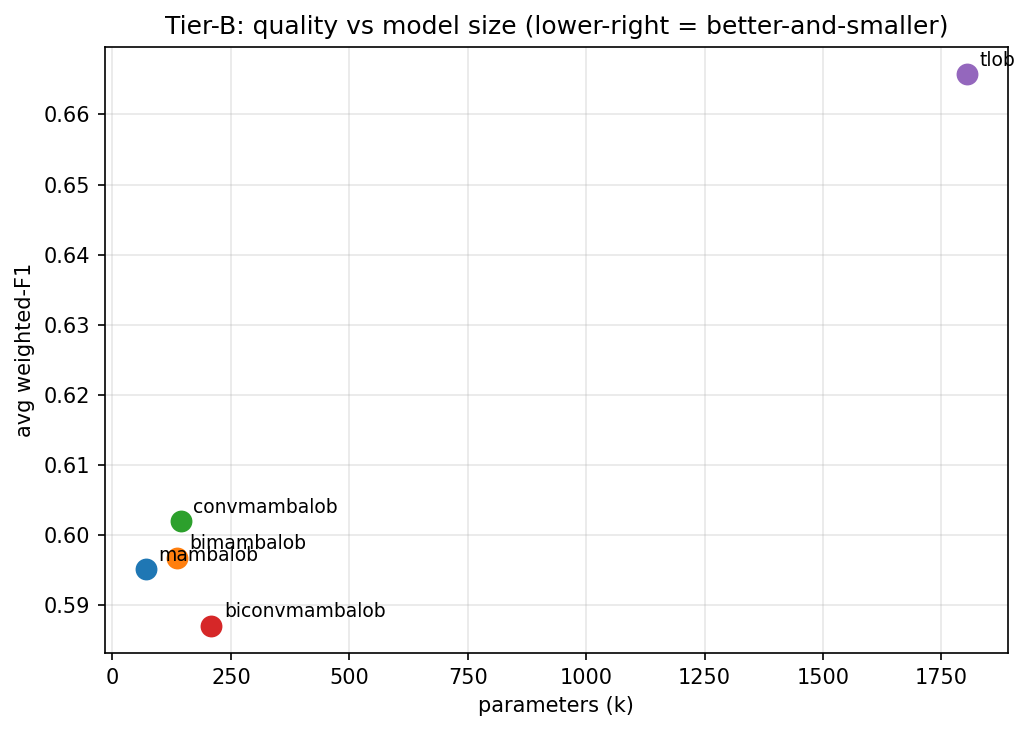
\includegraphics[width=\linewidth]{img/figures/architecture_fig_architecture.png}
\caption{Quality vs.\ model size. The Mamba family clusters near TLOB's accuracy at an order of magnitude
fewer parameters; the lower-right (better-and-smaller) is the design target.}
\label{fig:scatter}
\end{figure}

\subsection{Statistical rigour}
We re-ran the headline configurations over three seeds and tested each claim with paired across-seed tests
and per-sample bootstrap/McNemar tests (Table~\ref{tab:sig}). Microstructure feature engineering is
significant by every test ($+0.084$ weighted $F_1$, $p{=}0.001$), and is especially dramatic on BANKNIFTY,
where raw features collapse to $\approx$0.45 while engineered features reach $\approx$0.61. The ConvMambaLOB
gain is positive in direction but \emph{not} robust across seeds ($+0.005$, $p{=}0.25$), and TLOB's accuracy
lead is statistically significant ($p{<}0.001$). Hyperparameter optimisation gave only a modest gain, and the
tuned base MambaLOB --- at one layer and $d_{\mathrm{model}}{=}32$ --- matched the tuned ConvMambaLOB,
reinforcing that the efficient minimal SSM, not the hybrid, is the sweet spot. The proposed model is already
well-calibrated (test ECE $0.041$; NLL-optimal temperature $T{=}1.00$), so its probabilities are usable
directly. A class-imbalance study found class-weighted cross-entropy a sound default, with focal loss a
marginal alternative at long horizons.

\begin{table}[t]
\centering\footnotesize
\caption{Significance (weighted $F_1$). Across-seed: paired $t$-test over 12 cells.}
\label{tab:sig}
\begin{tabular}{@{}lcc@{}}
\toprule
Claim & $\Delta$ ($p$) & Verdict \\
\midrule
Features (\texttt{all} vs \texttt{base40}) & $+0.084$ ($0.001$) & significant \\
ConvMambaLOB vs MambaLOB & $+0.005$ ($0.25$) & not robust \\
Mamba/Conv vs TLOB       & $-0.07$ ($<0.001$) & TLOB ahead \\
\bottomrule
\end{tabular}
\end{table}

\subsection{Efficiency}
The motivating advantage of the SSM is its scaling. Figure~\ref{fig:scaling} contrasts TLOB's $O(L^2)$
attention with MambaLOB's $O(L)$ scan: MambaLOB's parameter count is constant in $L$ and its memory/latency
grow linearly, while TLOB's grow quadratically. At $L{=}800$, MambaLOB is $\approx$31$\times$ faster, uses
$\approx$3.4$\times$ less memory, and has $\approx$750$\times$ fewer parameters.

\begin{figure}[t]
\centering
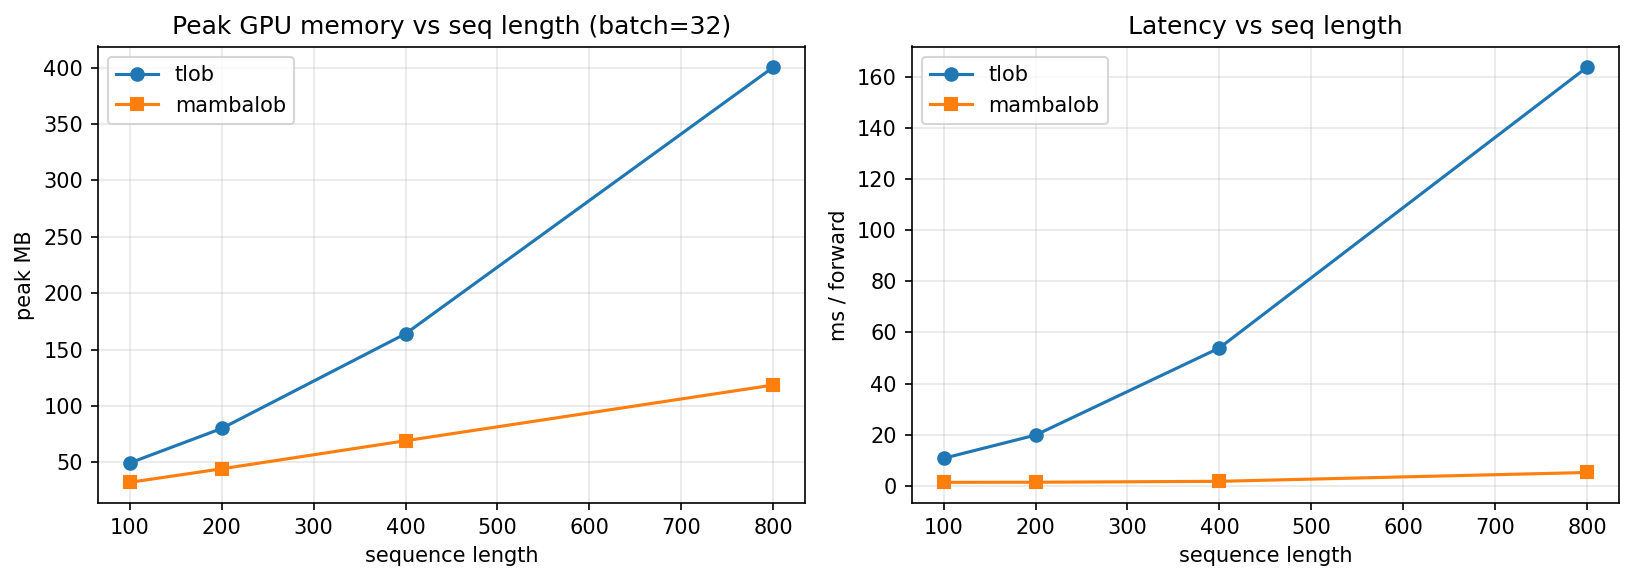
\includegraphics[width=\linewidth]{img/figures/mamba_fig_scaling_tlob_vs_mamba.png}
\caption{Sequence-length scaling: TLOB ($O(L^2)$) vs.\ MambaLOB ($O(L)$). The gap widens sharply with $L$.}
\label{fig:scaling}
\end{figure}

% =====================================================================
\section{Discussion and Conclusion}
\subsection{Discussion}
\textit{Interpretation of key findings.} Across reproduction, transfer, and a multi-seed rigour study, the
consistent story is that the contribution of the selective-SSM models is \emph{efficiency}, not accuracy: a
tiny MambaLOB recovers most of the transformer's quality at $12$--$25\times$ fewer parameters and linear-time
scaling, but TLOB's accuracy lead is real and significant. The largest \emph{significant} improvement on the
Indian market comes not from architecture but from \emph{microstructure feature engineering} --- the
engineered channels are what make the weaker NSE signal learnable.

\textit{Limitations.} The stored feed is a near-regular $\approx$0.4\,s snapshot stream rather than
tick-by-tick data; the NSE sample spans a single month; and the architecture gains, while directionally
positive, are within seed noise. These temper any claim of broad generalisation.

\textit{Future work.} A spread-relative (transaction-cost) labelling study, a cost-aware backtest with the
calibrated probabilities, and walk-forward robustness across more months and instruments.

\subsection{Conclusion}
We built the first ML-ready NSE index-futures LOB dataset through a full reverse-engineering and cloud
data-engineering effort, reproduced the standard deep LOB baselines, introduced MambaLOB and ConvMambaLOB, and
evaluated everything honestly with multi-seed significance, calibration, and hyperparameter optimisation. The
result is a clear efficiency--accuracy trade-off and a significant microstructure-feature effect, providing a
reproducible foundation for LOB modelling on Indian index futures.

\begin{footnotesize}
\bibliographystyle{plain}
\bibliography{references}
\end{footnotesize}

\end{document}
